Базовым методом оптимизации является спуск по координатам функции в направлении антиградиента. 
В условиях достаточной гладкости и выпуклости оптимизируемой функции такой метод позволяет находить глобальный максимум. 
В практических постановках функции не всегда удовлетворяют заданным условиями, что приводит к затуханию градиента 
в локальных минимумах. Исследователи разрешают проблему, модифицируя методы за счет использования моментов
и усреднения траектории.

\textit{Определение:} \textbf{Метод градиентного спуска} --- численный метод нахождения экстремума функции, использующий
в схеме градиент оптимизируемой функции:
\begin{equation}
    x_{t+1} = x_t - f(\nabla L(x_t)).
\end{equation}

Б. Т. Поляк показал \cite{polyak1990new}, что для функции с $L$-липшицевым градиентом оптимальной будет разностная схема: 
\begin{equation}
    x^{k+1} = x^k - \frac{1}{L} \nabla f(x^K)
    \label{simple_grad}
\end{equation}

В этом случае ошибка будет асимптотически линейно убывать с числом шагов $\frac{1}{N}$:
\begin{equation}
    f(x^N) -f(x_*) \le \frac{L R^2}{N},
\end{equation}
где $R=\| x^0 - x_* \|_2$. 

Докажем этот факт, используя $\mu$-выпуклость и $L$-гладкость функции.

\textit{\textbf{Теорема:} О простейшей схеме градиентного спуска} Пусть необходимо задать $x_*=\text{arg} \min_x f(x)$, где $f$ --- $L$-гладкая и
и $\mu$ -гладкая, тогда градиентный метод \ref{simple_grad} имеет линейную скорость сходимости.

\textit{Доказательство:} Ввиду L-гладкости функции $f$
\begin{equation}
    f(x^{k+1}) \le f(x^k) + <\nabla f(x^k), x^{k+1} -x^k> +\frac{L}{2} \|x^{k+1}-x^k\|_2^2
\end{equation}
Тогда:
\begin{equation}
    f(x^{k+1}) \le f(x^k) - \frac{1}{2L} \| \nabla f(x^k) \|^2_2
\end{equation}
С другой стороны из $\mu$-выпуклости получаем:
\begin{equation}
    f(x^{k+1}) \le f(x^k) - \frac{1}{2\mu} \| \nabla f(x^k) \|^2_2.
\end{equation}
Объединяя выражения получаем:
\begin{equation}
    f(x^{k+1}) -f(x_*) \le \left(1-\frac{\mu}{L}\right) (f(x^k)-f(x_*)).
\end{equation}
Рекурсивное применение неравенства задает:
\begin{equation}
    f(x^k) - f(x_*) \le (1-\frac{\mu}{L})^k (f(x^0)-f(x_*))
\end{equation}
$\blacksquare$

На практике линейная сходимость может быть недостаточна, потому разрабатываются продвинутые методы, выполняющий спуск с
асимптотически квадратичным убыванием ошибки. К таким методам относятся методы сопряженных градиентов и 
метод тяжелого шарика Поляка.

Схема выполнения нового шага по методу сопряженных градиентов выглядит как:
\begin{equation}
    x^{k+1} = x^k - \alpha_k \nabla f(x^k) + \beta_k (x^k -x^{k-1}),
\end{equation}
где $(\alpha_k,\beta_k) \in arg \min_{\alpha,\beta} f(x^k - \alpha \nabla f(x^k) + \beta (x^k -x^{k-1}))$
дает оценку скорости сходимости как:
\begin{equation}
    f(x^N) -f(x_*) \le \frac{L R^2}{N^2}
\end{equation}

Метод тяжелого шарика Поляка учитывает значение с предыдущего шага $x^{k-1}$. Оптимальная численная схема
для $\mu$-выпуклой функции с $L$-гладким градиентом запишется как:
\begin{equation}
    x^{k+1} = x^k - \frac{4}{(\sqrt{L}+ \sqrt{\mu})^2} \nabla f(x^k) + \frac{(\sqrt{L} -\sqrt{\mu})^2}{(\sqrt{L} +\sqrt{\mu})^2} (x^k - x^{k-1})
\end{equation}

\begin{figure}[h]
    \centering
    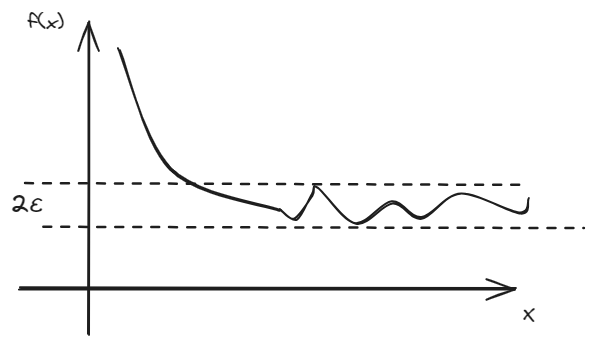
\includegraphics[width=0.5\textwidth]{assets/math/optimization/stability.excalidraw.png}
    \caption{Устойчивость метода при выходе на плато}
    \label{optimization}
\end{figure}

В приложении к машинному обучению известны также модификации метода тяжелого шарика:
\begin{enumerate}
    \item AdaGrad \cite{duchi2011adaptive} задает адаптивный шаг спуска для каждого параметра $i$
    с учетом индивидуального градиента $\nabla_{\theta_i} \mathcal{L}(\theta_i)$:
        \begin{equation}
            \begin{aligned}
                &x_{t+1} = x_t - \frac{\eta}{\sqrt{g_t+\epsilon}} \cdot \nabla L(x_t) \\
                &g_{t+1} = g_t + \nabla_\theta \mathcal{L}(\theta)^2
            \end{aligned}
        \end{equation}
    Итерация начинается с $g_t=0$. Исследователи отмечают повышение эффективности метода в постановках с функциями распределения параметров 
    с тяжелыми хвостами.
    \item RMSProp \cite{krizhevsky2012imagenet} модификация метода скользящим средним по параметру накопления градиента:
        \begin{equation}
            \begin{aligned}
                &x_{t+1} = x_t - \frac{\eta}{\sqrt{g_t+\epsilon}} \cdot \nabla L(x_t) \\
                &g_t = \mu g_{t+1} + (1-\mu)\nabla L(x_t) \cdot \nabla \mathcal{L}(\theta)^2
            \end{aligned}
        \end{equation}
    \item Adam \cite{kingma2014adam} --- метод совмещающий скользящее среднее по градиенту и параметру накопления градиента:
        \begin{equation}
            \begin{aligned}
                &x_{t+1} = x_t - \frac{\eta}{\frac{\sqrt{g_t+\epsilon}}{1-\mu^t}} \cdot \frac{v_{t+1}}{1-\beta^t} \\
                &v_{t+1} = \beta v_t + (1-\beta) \nabla L(x_t) \\
                &g_t = \mu g_{t-1} + (1-\mu)\nabla L(x_t) \cdot \nabla  L(x_t)
            \end{aligned}
        \end{equation}
    Отметим, что метод не обязательно сходится даже в выпуклой постановке \cite{reddi2019convergence}. Тем не менее на практике полученный
    алгоритм, как правило, обладает наилучшими показателями сходимости.
\end{enumerate}


